\documentclass[12pt,a4paper]{article} 
\usepackage{graphicx}
\usepackage{amsmath}
\usepackage[utf8x]{inputenc} 
\usepackage[encapsulated]{CJK}
\usepackage{textcomp} 
\usepackage{hyperref}
\usepackage{float}
\usepackage[]{algorithm2e}
\usepackage{algpseudocode}
\begin{CJK}{UTF8}{bsmi} 
	\title{Homework 5 - Stationary Gaussian white process and linear transform } 
	\author{Professor : Ren Jung Chang 張仁宗 \\Student : N16066176 Chen Wei Yu 余振瑋} 
	\date{Oct 23 2017}
\begin{document}
	\maketitle	 
	\tableofcontents
	\listoffigures
	\begin{abstract}
		Homework 5 is designed for discussing the property of the Gaussian white process by using the autocorrelation function or the other method. After discussion about the autocorrelation and the other method of the Gaussian wite process, we also discuss the linear transform properties of the white noise. With the linear transform, we can apply the filter theorem dealing with the white noise. After removing some signal from the white noise by the filter, we will discuss the output signal by the statinoary test.
	\end{abstract}
	\section{List of symbols}
	\begin{itemize}
		\item $G_{xx}$ : autospectral density function(one-sided)
		\item $S_{xx}$ : autospectral density function(two-sided)
		\item $S_{xy}$ : crossspectral density function(two-sided)
		\item $R_{xx}$ : autocorrelation function
		\item $\delta(t)$ : Dirac delta function
		\item $\mu$ : mean
		\item $\sigma$ : standard deviation
		\item $\sigma^{2}$ : variance
	\end{itemize}
	\section{Problem}
	\subsection{Problem 1}
	\subsubsection{Describtion}
	\paragraph{Use}Matlab to generate and display a Gaussian white process and verify the white property by using autocorrelation function in Matlab.
	\subsubsection{Answer}
	\paragraph{We} define the Gaussian white process at first. The Gaussian process is defined as below:\\
	\begin{itemize}
		\item Continous time : X(t) is a Gaussian stochastic process if and only if $X=[x(t_{1})\cdots x(t_{k})]^{T}$ is a Gaussian random vector for an arbitary integer $k>0$ and any time instants.
		\item Discrete sequence : $X_{n}$ is a Gaussain sequence if and only if $X=[x_{n_{1}}\cdots x_{n_{k}}]^{T}$ is a Gaussian random vector for an arbitary integer $k>0$ and any time instants.
	\end{itemize}\cite{Book2}
	\paragraph{The}techanical term 'white' means the 'white noise( process ).' There are some propertise of the white noise as below.\cite{Book1}
	\begin{itemize}
		\item 
		\begin{equation}
			G_{xx}(f)=a \quad only\:for f\geq0 
		\end{equation}
		\item 
		\begin{equation}
			S_{xx}(f)=(a/2) \: for \: all \: f
		\end{equation}
		\item 
		\begin{equation}
			R_{xx}(\tau)=(a/2)\,\delta(\tau)
		\end{equation}
		\item 
		\begin{equation}
			\int_{0}^{\infty}G_{xx}(f)df=\infty=R_{xx}(0)
		\end{equation}
	\end{itemize} 


	\paragraph{Which}$R_{xx}$ means the autocorrelation of the random number $x$. $S_{xx}(f)$ is the two-sided autospectral density functions which is defined for $f\,\in\,(-\infty,\infty)$ by the Fourier transform of the random variable $x$. The approach is called as the Wiener–Khintchine theorem\cite{Net1}.$G_{xx}$ is the one-side autospectral density function where $0 \leq f < \infty$. From equation $1\sim 2$ show that white noise has an infinite mean square vlaue. So theoretical white noise cannot be Gaussian process because that Gaussian process has finite mean square value. However,the Gaussian white process means that the PDF(probability density function) of the zero mean white noise is Gaussian destribution.
	\begin{figure}[H]
		\begin{center}
			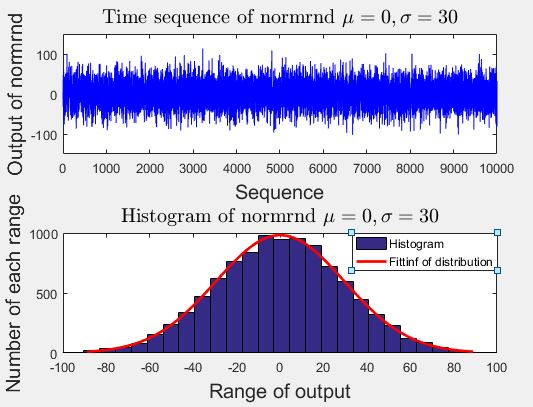
\includegraphics[scale=0.5]{Problem1a}
			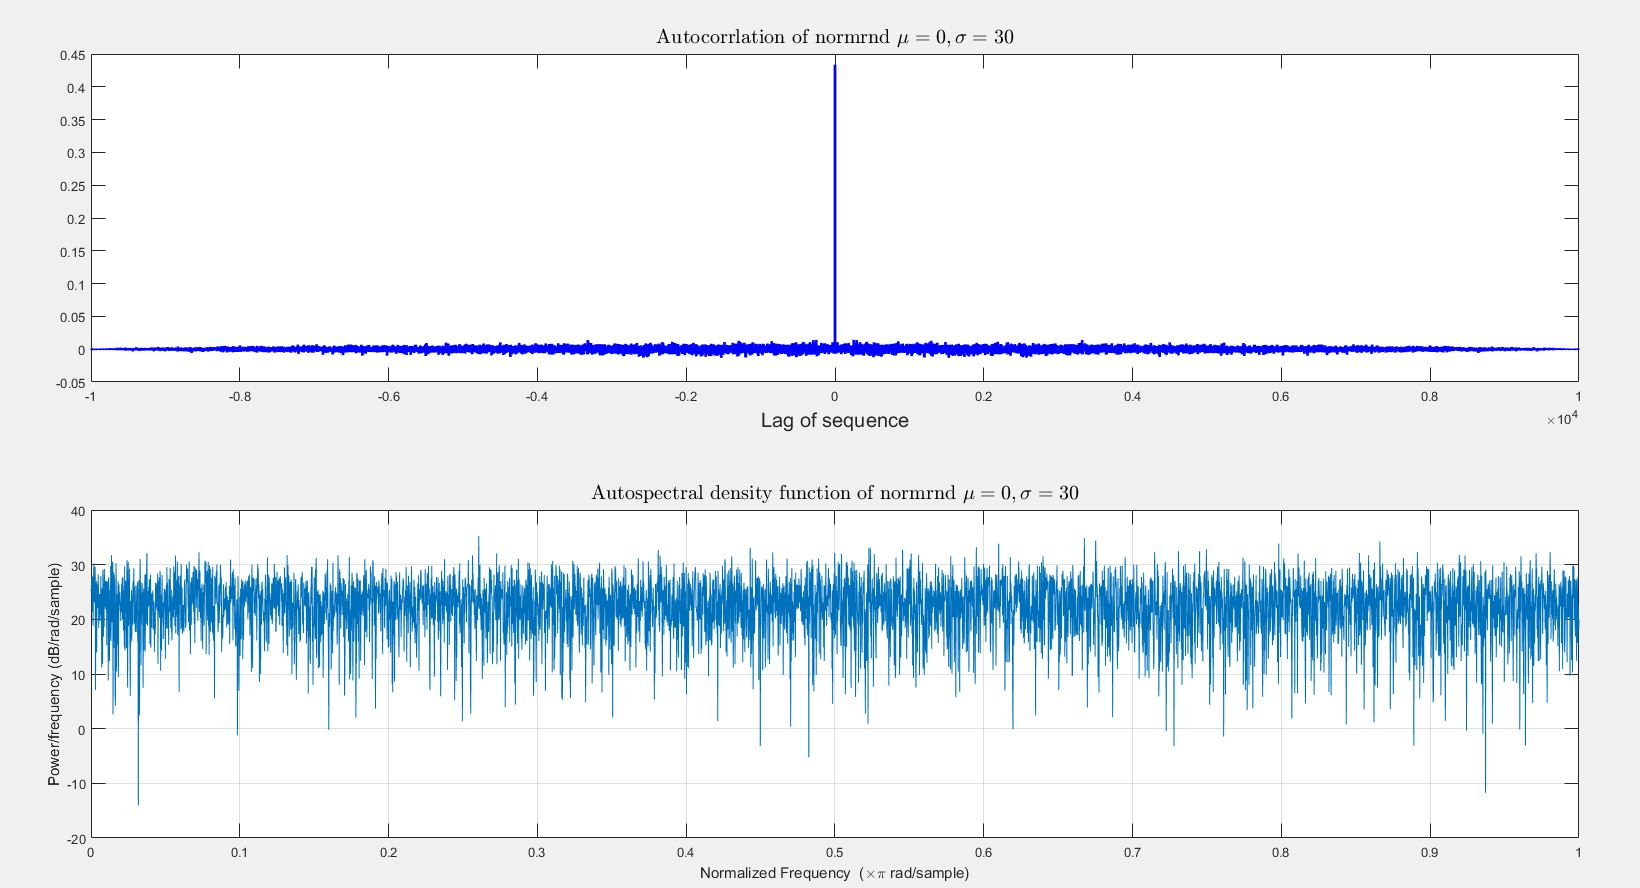
\includegraphics[scale=0.4]{Problem1a2}
		\end{center}
		\caption[Properties of the Gaussian white process generated by the naive matlab function]{Fisrt figure is the time sequence with the output from the naive matlab function normrnd. Second one is the histogram and the fitting diagram.Third figure is the autocorrelation of the random sequence.Final one is the autospectral density function.}
	\end{figure}
	\begin{figure}[H]
		\begin{center}
			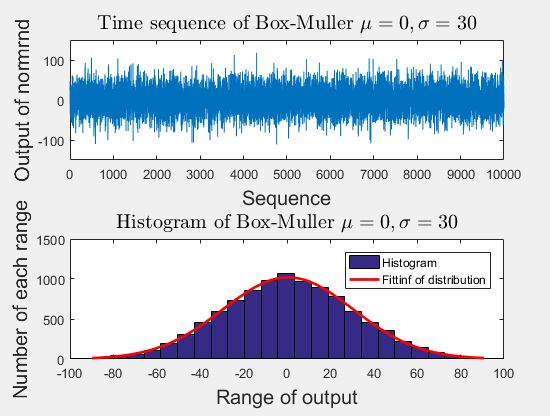
\includegraphics[scale=0.5]{Problem1b}
			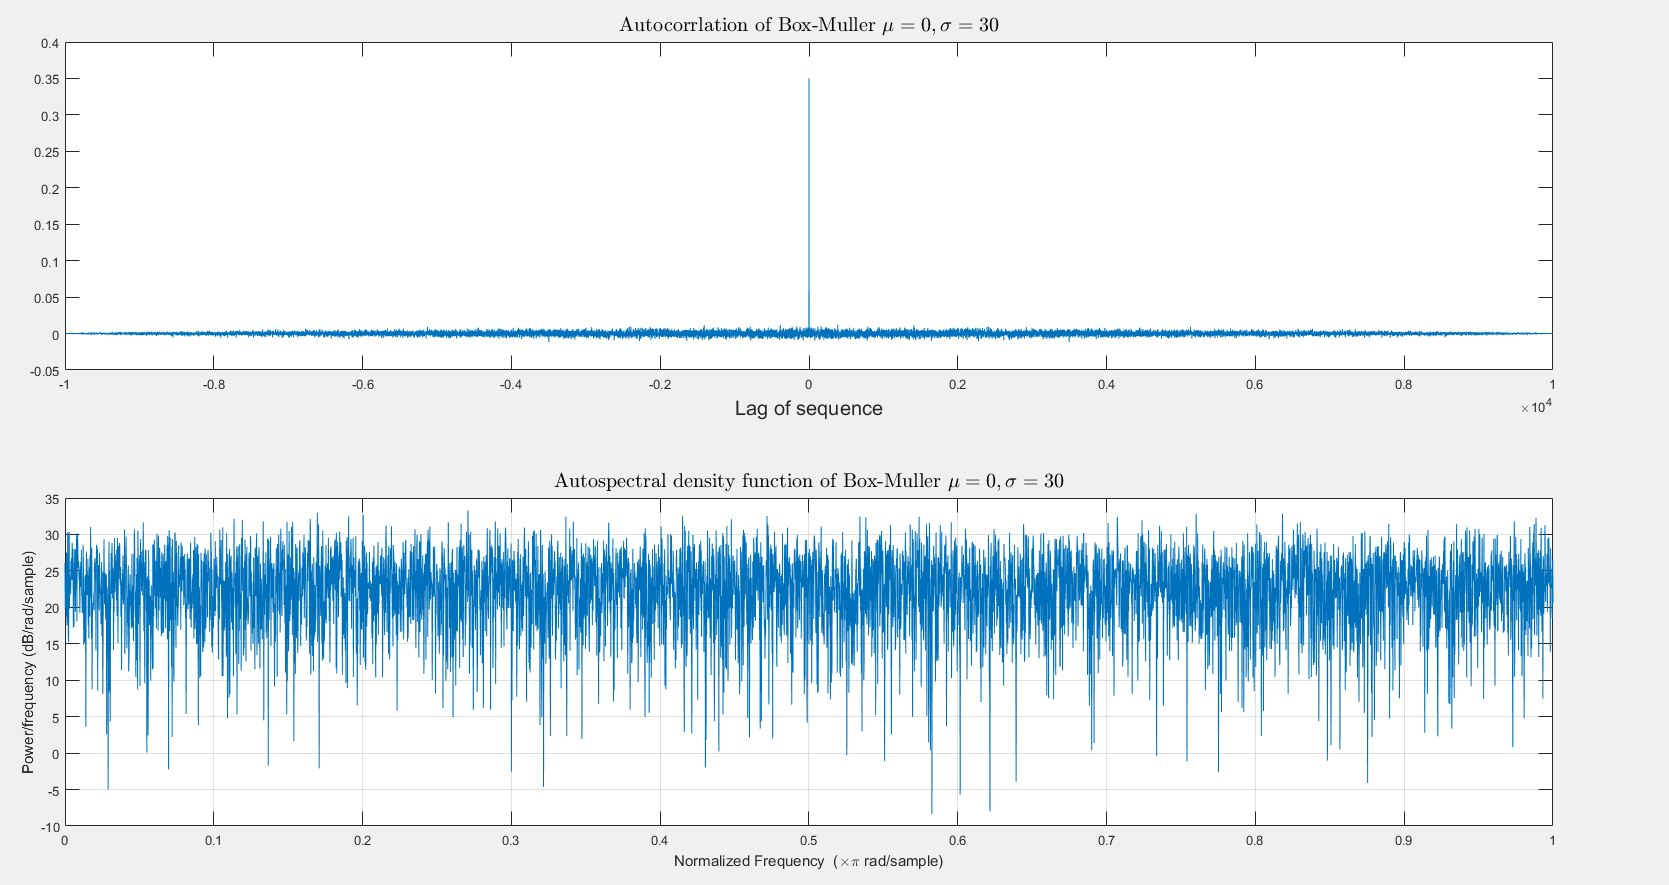
\includegraphics[scale=0.4]{Problem1b2}
		\end{center}
		\caption[Properties of the Gaussian white process generated by the Box-M\"{u}ller method]{Fisrt figure is the time sequence with the output from the Box-M\"{u}ller method(from previous homework). Second one is the histogram and the fitting diagram.Third figure is the autocorrelation of the random sequence.Final one is the autospectral density function.}
	\end{figure}
	\subsection{Problem 2}
		\subsubsection{Describtion}
			\paragraph{Generate}a random response for 1st and 2nd-order low-pass filter 
			with input of Gaussian white process. The input to the filter by 
			using randn() in Matlab should be divided by the square root of 
			step size in time sequence. The transfer function of the 1st and 
			2nd-order filters are given as $TF_{1}=\frac{1}{2s+1}$ and $TF_{2}=\frac{0.25}{s^{2}+0.7071s+0.25}$ , respectively.
		\subsubsection{Answer}
			\paragraph{We}discuss the linear transformation of random process at fist. If there is an arbitrary random sequence $\{x_{k}(t)\}$ and a transform operator $A:t \to v$ which will let the sample function $\{x_{k}(t)\}$ map into $\{y_{k}(v)\}$.
			If the transform operator is linear(which means that it is additive,inversible,homogeneous), then the image of $x_{k}(t)$ is $y_{k}(v)$  which has the following properties.
			\begin{enumerate}
				\item If $x(t)$ is from a weakly(strongly) stationary random process and if the operator $A$ is linear and time-invariant, then $y(v)=A[x(t)]$ will form a weakly(strongly) stationary random process.
				\item If $x(t)$ follows a Gaussian distribution and the operator $A$ is linear, then $y(v)=A[x(t)]$ will also follow a Gaussian distribution.
			\end{enumerate}
			\paragraph{If}a stationary random signal input to a LTI system, it can represnt bt the below figure. \\
			\begin{figure}[H]
				\centering
				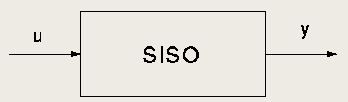
\includegraphics[scale=1.0]{SISO}
				\caption[SISO system]{The input of the SISO system is generally denoted as the symbol $u$ and the output is $y.$However,we use the input signal denoted as $x$ instead of $u$ for convince.}
			\end{figure}
			\paragraph{The}output $y(t)$ is defined as $y(t)=\int_{0}^{\infty}h(\tau)x(t-\tau)d\tau$ where $h(\tau)=0 \quad for \quad\tau<0.$ After some caculations, we can get the two side spectrum ralations as below:\\
			\begin{itemize}
				\item Input/Output autospectrum relation : 
					\begin{equation}
						S_{yy}(f)=|H(f)|^{2}S_{xx}(f)
					\end{equation}
				\item Input/Output cross-spectrum relation : 
					\begin{equation}
						S_{xy}(f)=H(f)S_{xx}(f)
					\end{equation}
			\end{itemize}
			\subparagraph{And}the one-side spectral density functions $G_{xx}(f),G_{yy}(f),G_{xy}(f)\,,where\, G(f)=2S(f)\,for\,f\geq0$\\
			\begin{itemize}
				\item
					\begin{equation}
						G_{yy}=|H(f)|^{2}G_{xx}(f)
					\end{equation}
				\item 
					\begin{equation}
						G_{xy}(f)=H(f)G_{xx}(f)=|G_{xy}(f)|e^{-j\theta^{xy}(f)}
					\end{equation}
				\item 
					\begin{equation}
						H(f)=|H(f)|e^{-j\theta(f)}
					\end{equation}
			\end{itemize}
			\paragraph{We} discuss the frequency response by Bode plot of each filter.\\
			\begin{figure}[H]
				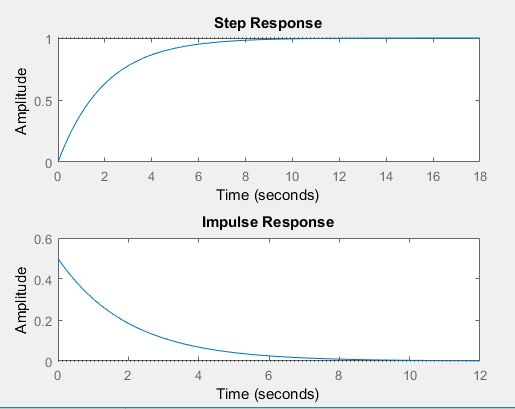
\includegraphics[scale=0.58]{Problem2a}
				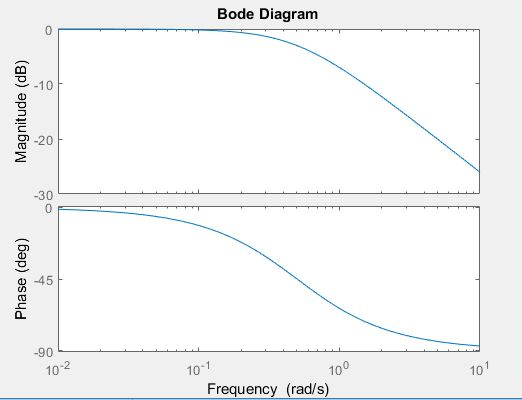
\includegraphics[scale=0.6]{Problem2b}
				\caption[Properties of the fisrt filter]{The left two figures are the step and the impulse response of the $TF_{1}=\frac{1}{2s+1}$. The right side are the frequency responses and we can find that the corrner frequency is close to $0.4\, rad/s.$ }
			\end{figure}
			\begin{figure}[H]
				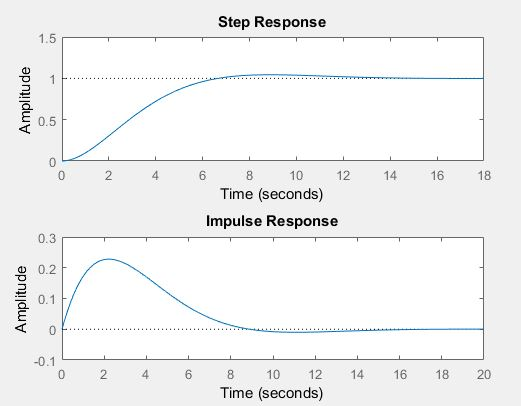
\includegraphics[scale=0.55]{Problem2c}
				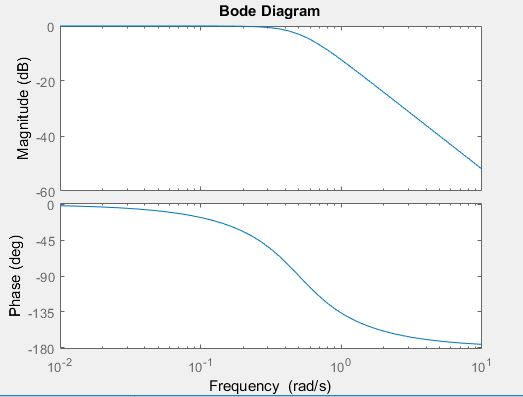
\includegraphics[scale=0.56]{Problem2d}
				\caption[Properties of the second filter]{The left two figures are the step and the impulse response of the $TF_{2}=\frac{0.25}{s^{2}=0.7071s+0.25}$. The right side are the frequency responses. The right side are the frequency responses and we can find that the corrner frequency is close to $0.3\sim0.4\, rad/s.$}
			\end{figure}
			\begin{figure}[H]
				\centering
				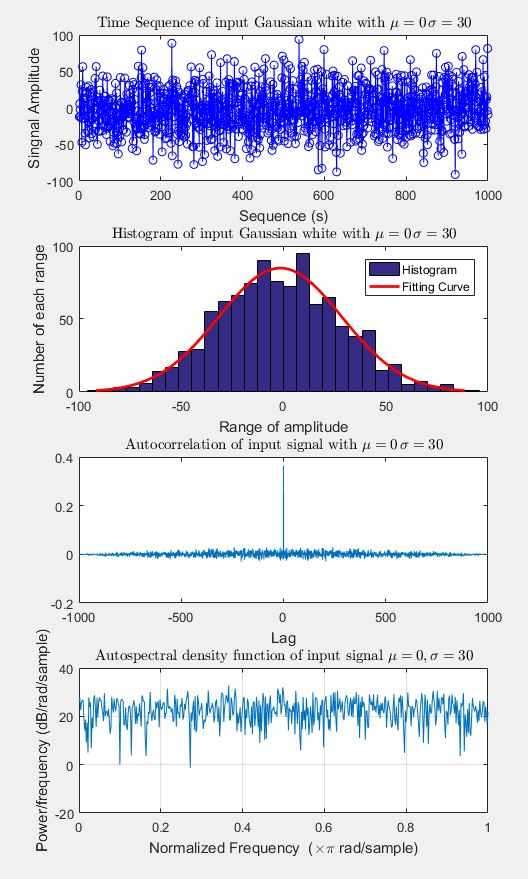
\includegraphics[scale=0.8]{Problem2e}
				\caption[Properties of the Gaussian white input]{First figure is the input amplitude of Gaussian white noise versus time sequences.The second one is the histogram of the input signal versus amplitude.The third is the auto-correlation of input signal.Final one is the autospectral density diagram.}
			\end{figure}
			\begin{figure}[H]
				\centering
				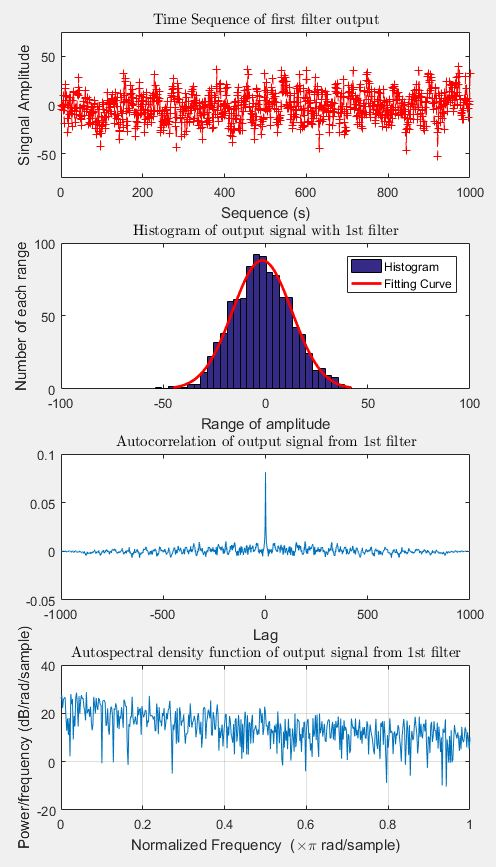
\includegraphics[scale=0.8]{Problem2f}
				\caption[Properties of the output signal from the 1st filter]{First figure is the amplitude of output signal from 1st filter versus time sequences.The second one is the histogram of the output signal versus amplitude.The third is the auto-correlation of output signal.Final one is the autospectral density diagram.We can see that the output signal start to decay approximately at $0.2\times\pi\simeq0.6\,rad/s.$ }
			\end{figure}
			\begin{figure}[H]
				\centering
				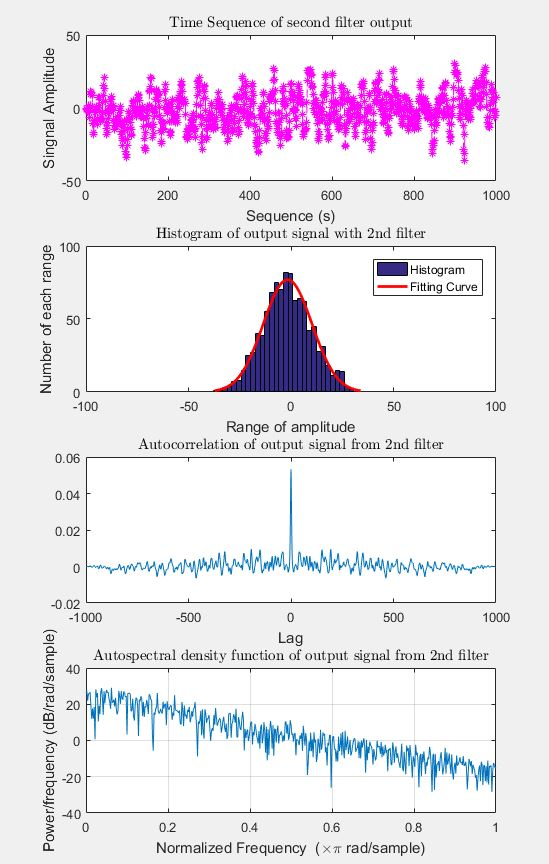
\includegraphics[scale=0.8]{Problem2g}
				\caption[Properties of the output signal from the 2nd filter]{First figure is the amplitude of output signal from 2nd filter versus time sequences.The second one is the histogram of the output signal versus amplitude.The third is the auto-correlation of output signal.Final one is the autospectral density diagram.We can see that the output signal start to decay approximately at $0.15\times\pi\simeq0.45\,rad/s.$}
			\end{figure}
			\begin{figure}[H]
				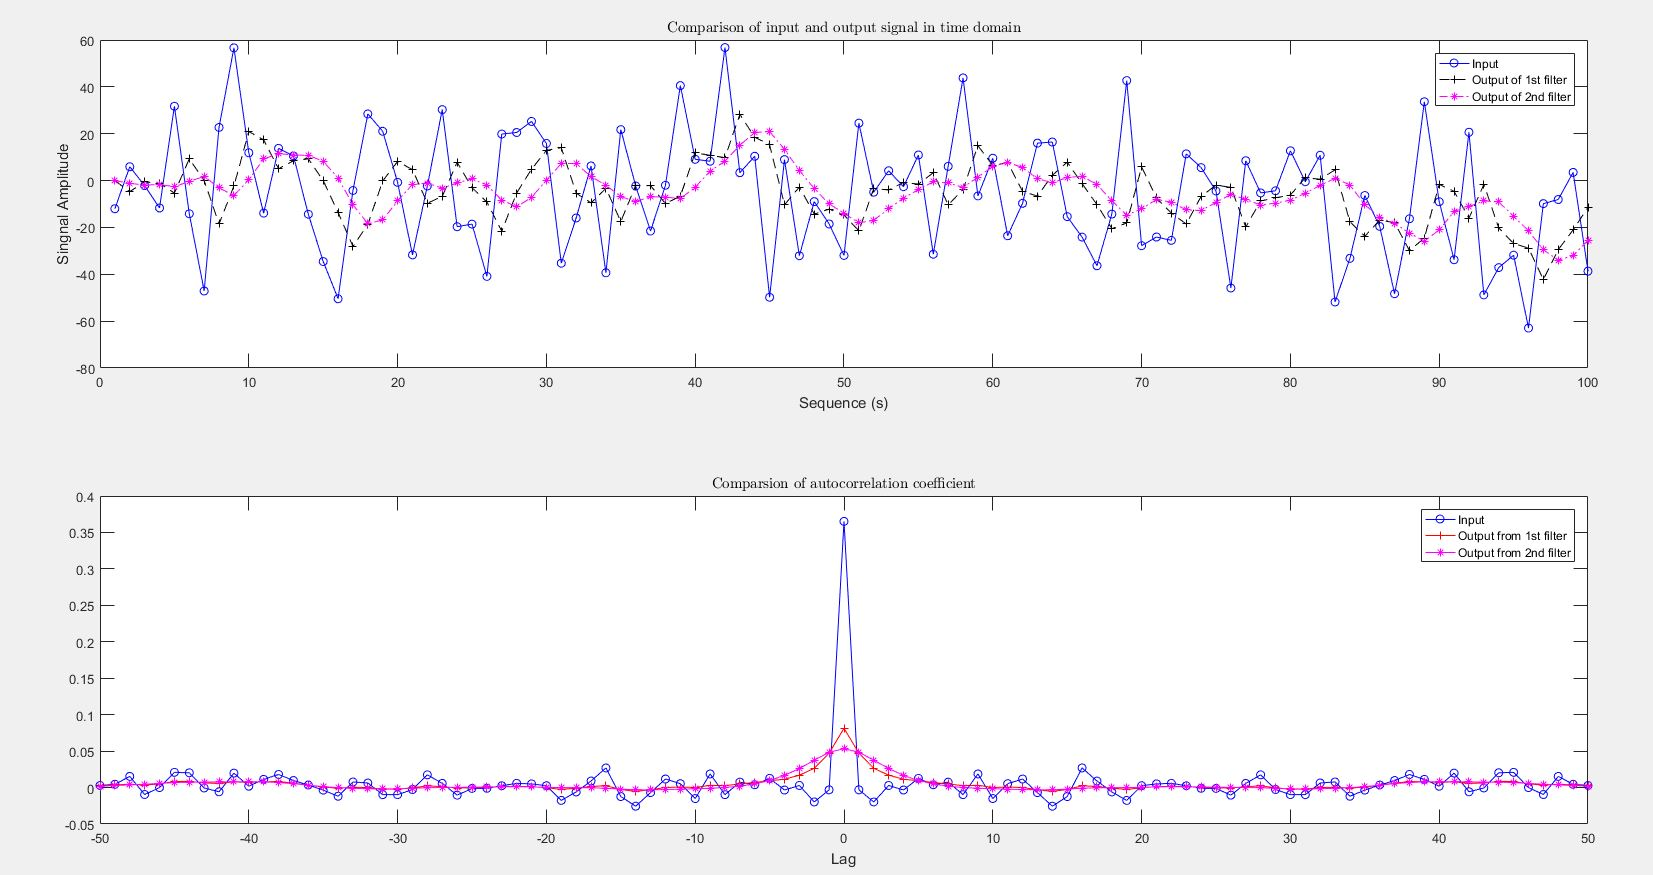
\includegraphics[scale=0.4]{Problem2h}
				\caption[Properties of input and output signal on time domain]{The first figure is the comparsion of the input and output signal on time domain.The second one is the comparsion of the autocorrelation function between the input and output signal.}
			\end{figure}
			\begin{figure}[H]
				\centering
				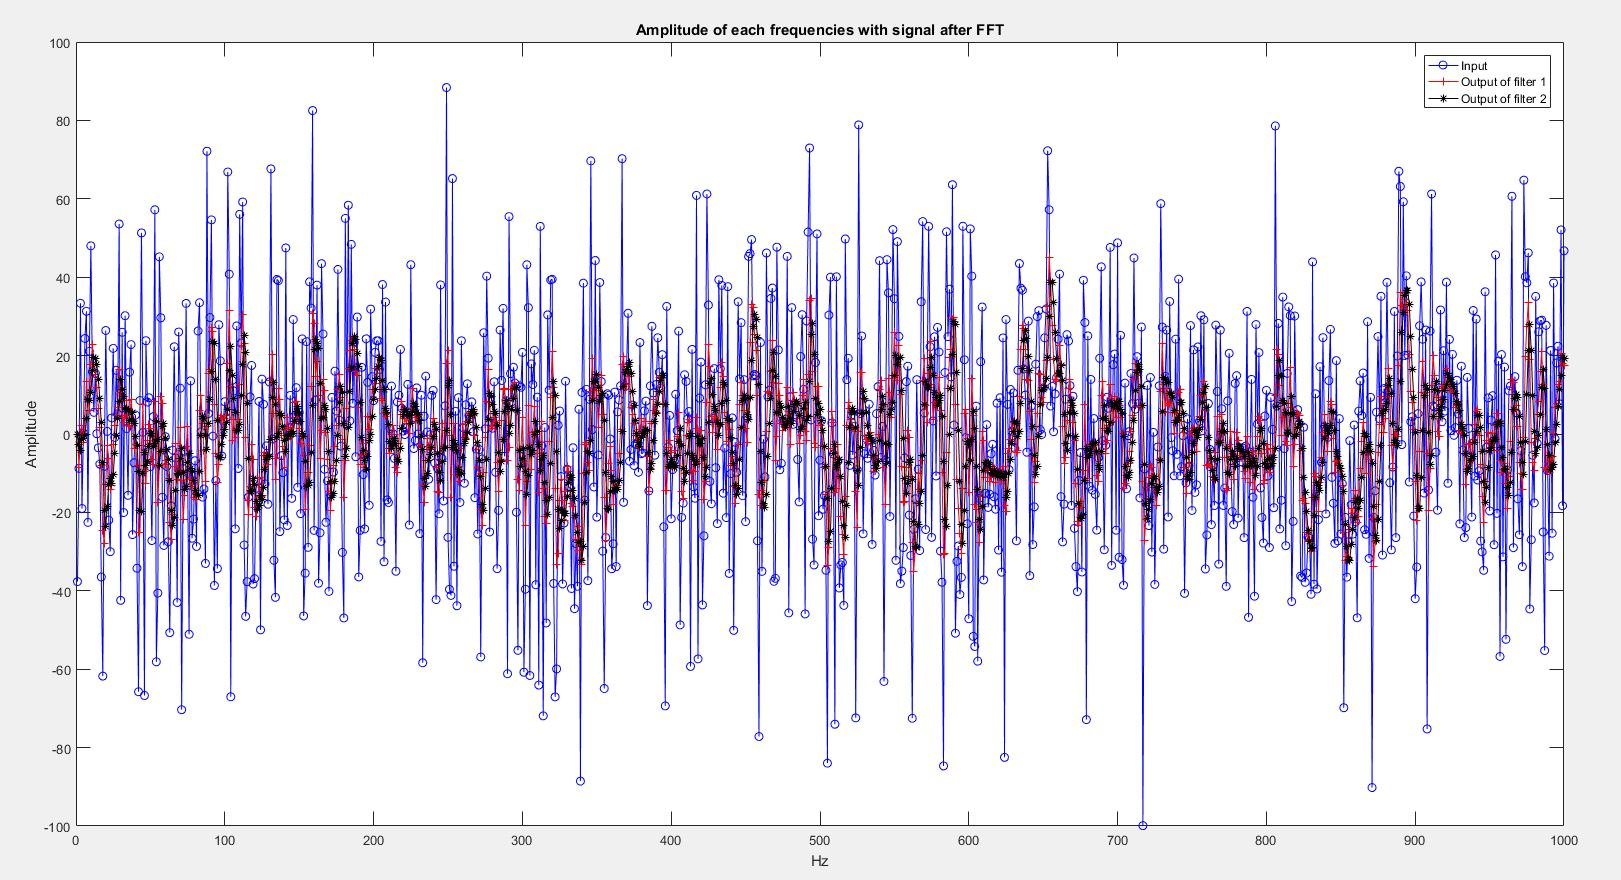
\includegraphics[scale=0.4]{Problem2i}
				\caption[FFT of random number on the frequency domain]{The figure is the comparsion between the amplitude of the input and output signal on frequency domain by FFT.}
			\end{figure}
			\begin{figure}[H]
				\centering
				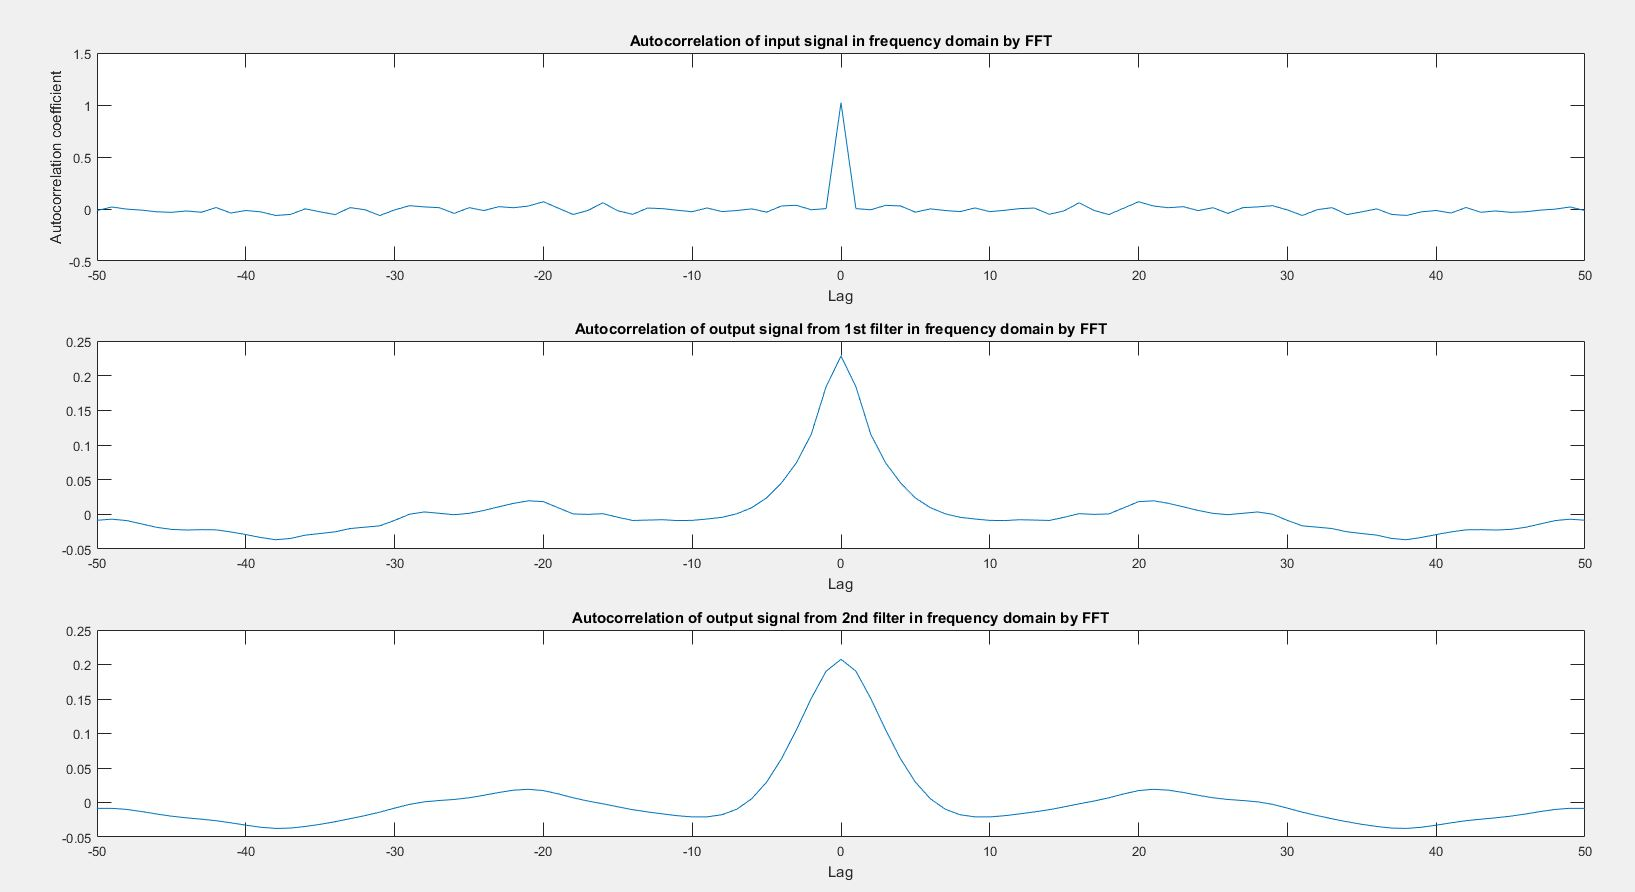
\includegraphics[scale=0.4]{Problem2j}
				\caption[Autocorrelation of the input and output signal on frequency doiman separately]{The figure is the autocorrelation of the input and output signal on frequency domain separately.}
			\end{figure}
			\begin{figure}[H]
				\centering
				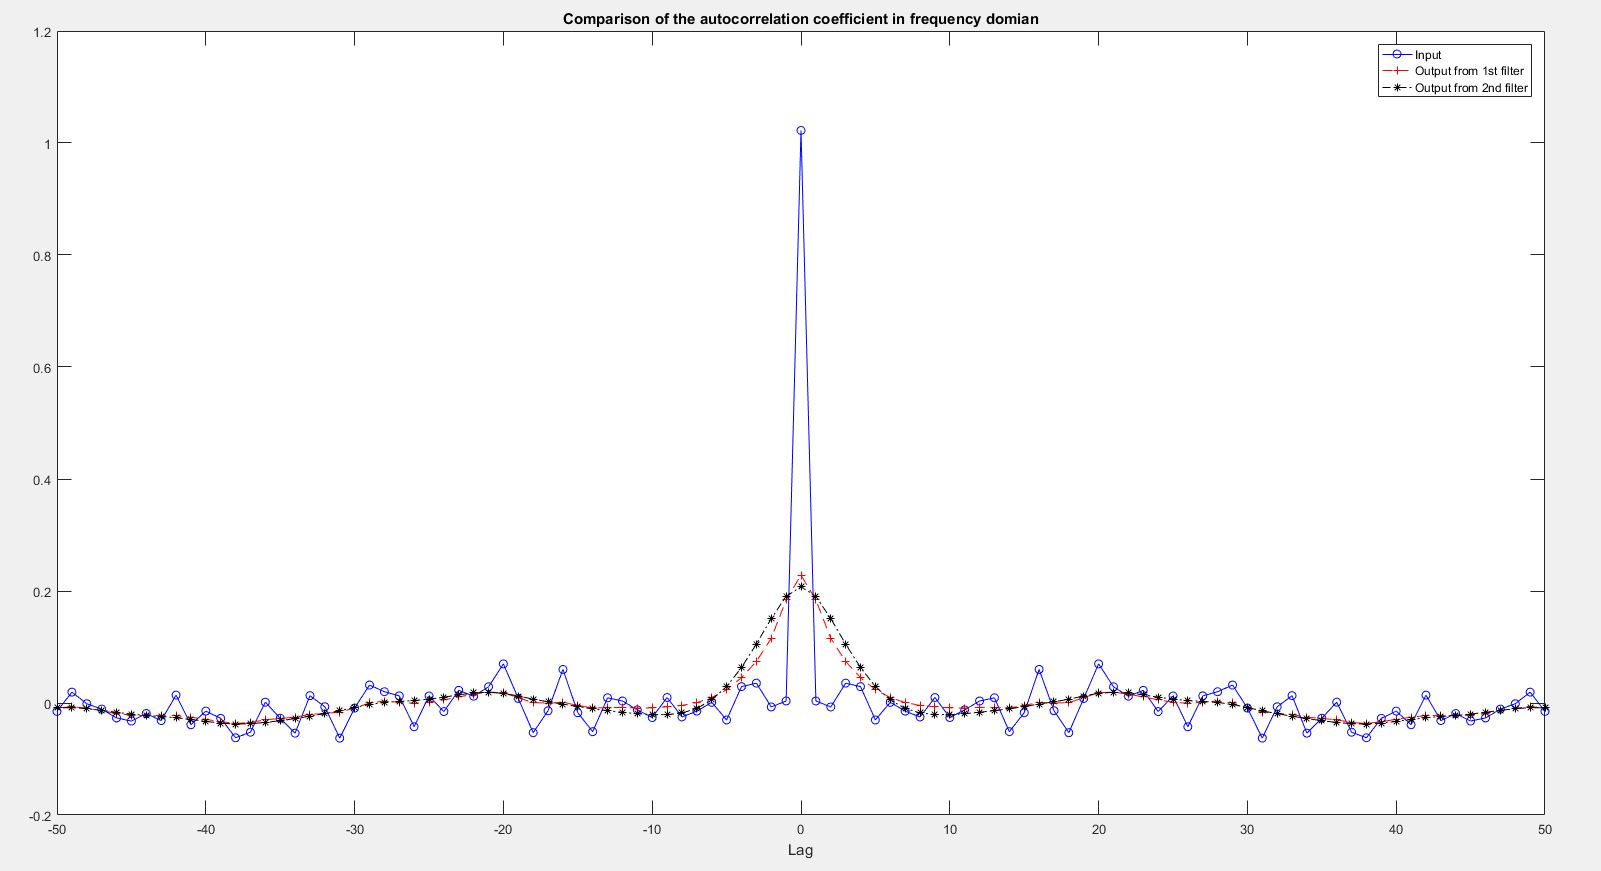
\includegraphics[scale=0.4]{Problem2k}
				\caption[Comparsion of the autocorrelation between the input and output signal on frequency doiman separately]{The figure is the comaprsion of the autocorrelation between the input and output signal on frequency domain.}
			\end{figure}
		\subsection{Problem 3}
			\subsubsection{Describtion}
				\paragraph{Discard} the nonstationary part and show that the response reaches weakly stationary through ensemble average by numerical verification. 
			\subsubsection{Answer}
				\paragraph{The}problem is designed for disgussed for the ergodic and statonary property.The strickly stationary is defined as the statictical properties likes mean,\\variance,standard deviation$\cdots$ are independent of time.The definition of the ergodic based on the book\cite{Book1} is defined as "the mean and the autocorrelation of the random data are independed of the different sample".A radom data is stationary ergodic means that the ensemble average equals to the time average. 
			\begin{figure}[H]
				\centering
				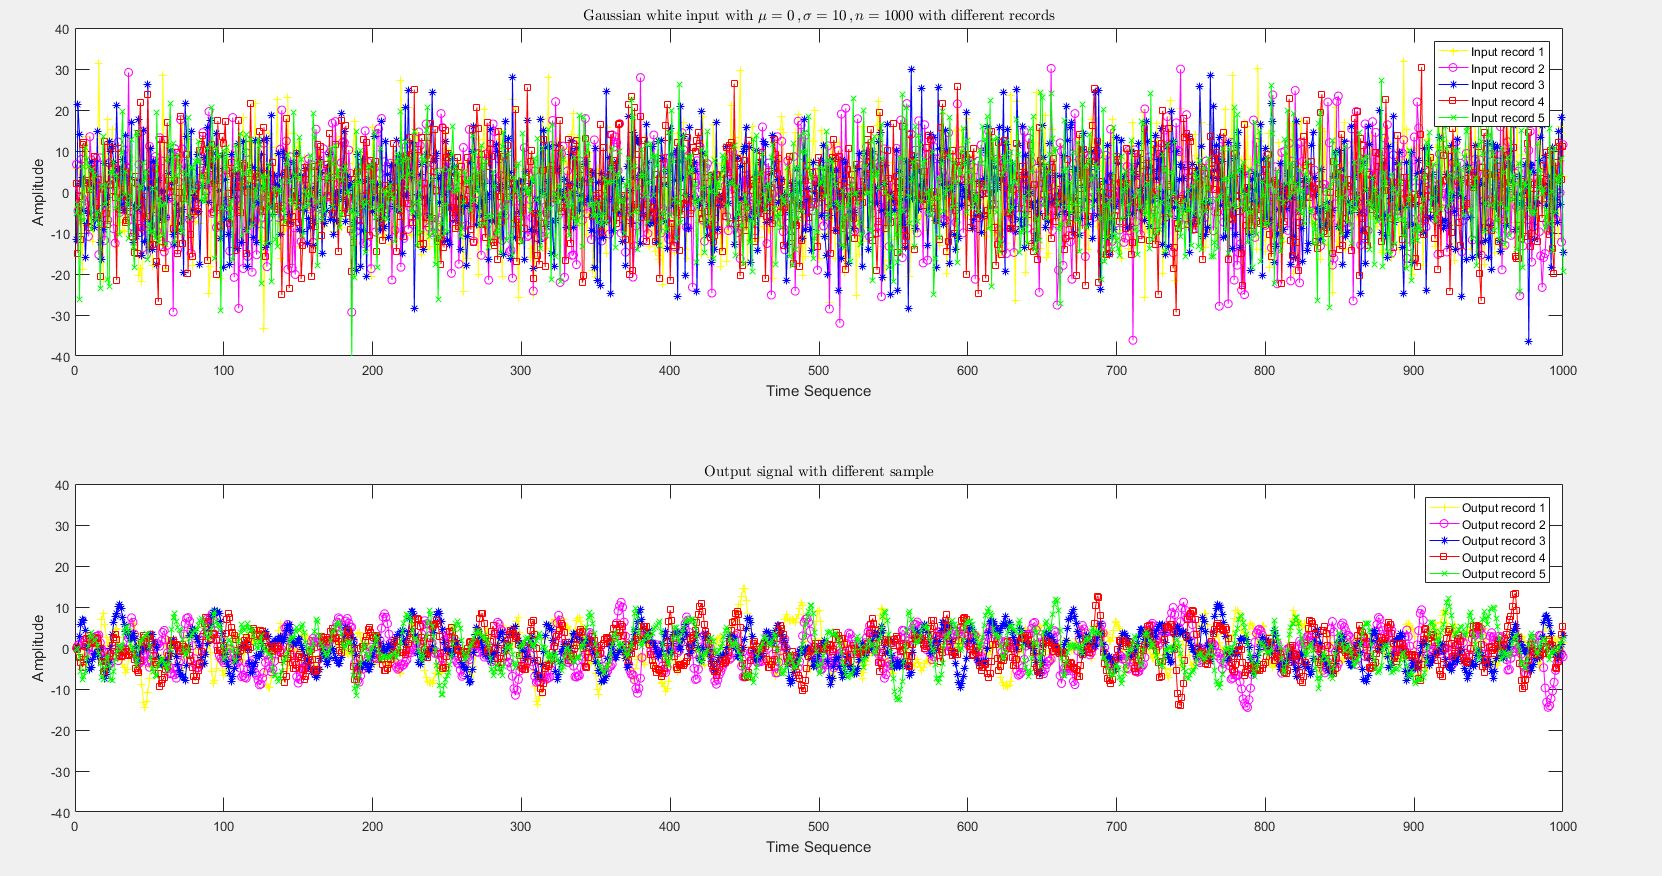
\includegraphics[scale=0.4]{Problem3a}
				\caption[Input and output signal with different records]{Input and output signal with different smaple records in time sequence $0\sim1000$ (The figure only displays first five sample records without showing the other 995 sample records.The number of the total sample records is 1000.)} 
			\end{figure}
			\begin{figure}[H]
				\centering
				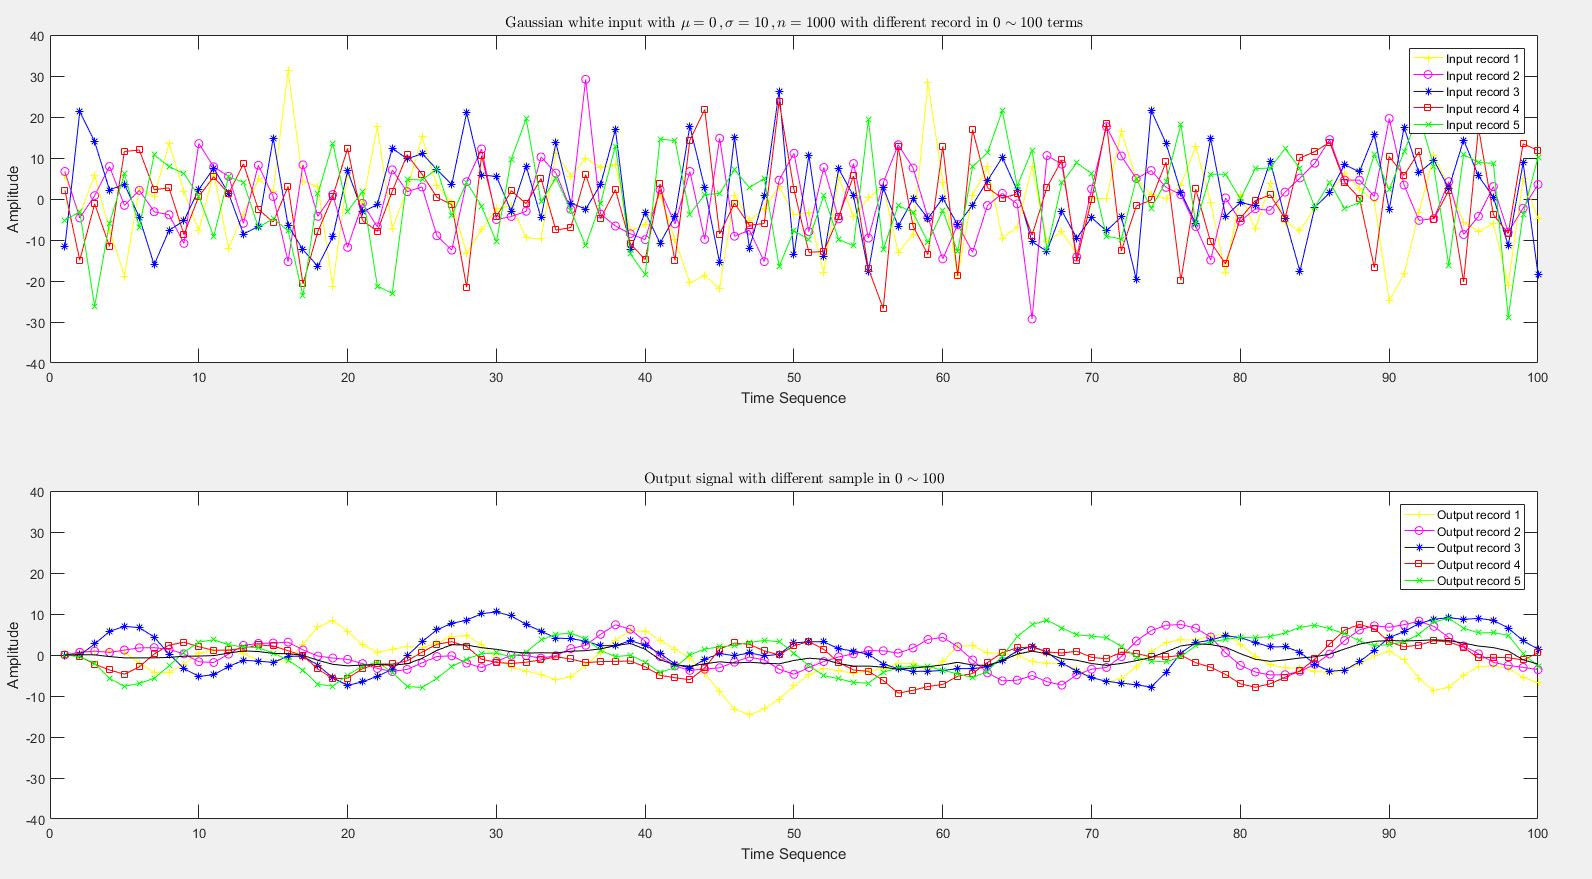
\includegraphics[scale=0.4]{Problem3b}
				\caption[Input and output signal with different records in time $0\sim100$]{Input and output signal with different records in time $0\sim100$ (The figure only displays first five sample records without showing the other 995 sample records.The number of the total sample records is 1000.)}
			\end{figure}
				\begin{figure}[H]
					\centering
					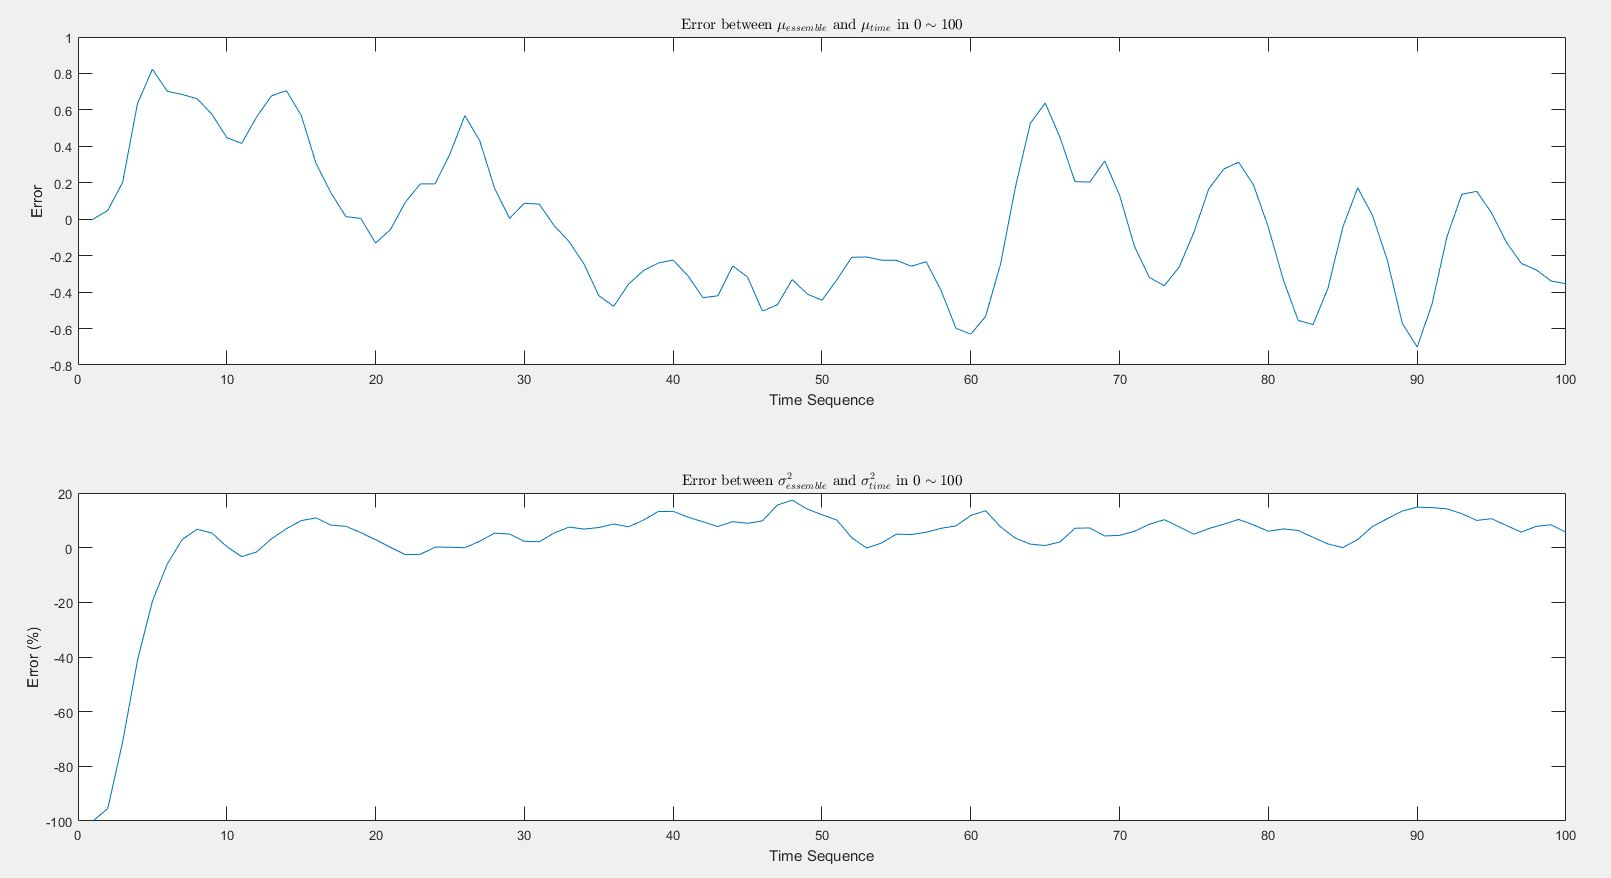
\includegraphics[scale=0.4]{Problem3c}
					\caption[Ensemble average and essemble variance with nostationary part]{We can see the output signal is not stationary by the second figure which is the difference of esemble variance and the time variance bsaed on the method $\frac{\sigma^{2}_{emsemble}-\sigma^{2}_{time}}{\sigma^{2}_{time}}$.The first one is the difference of ensemble average and time average based on the formula $\mu_{esemble}-\mu_{time}$.}
				\end{figure}
			\begin{figure}[H]
				\centering
				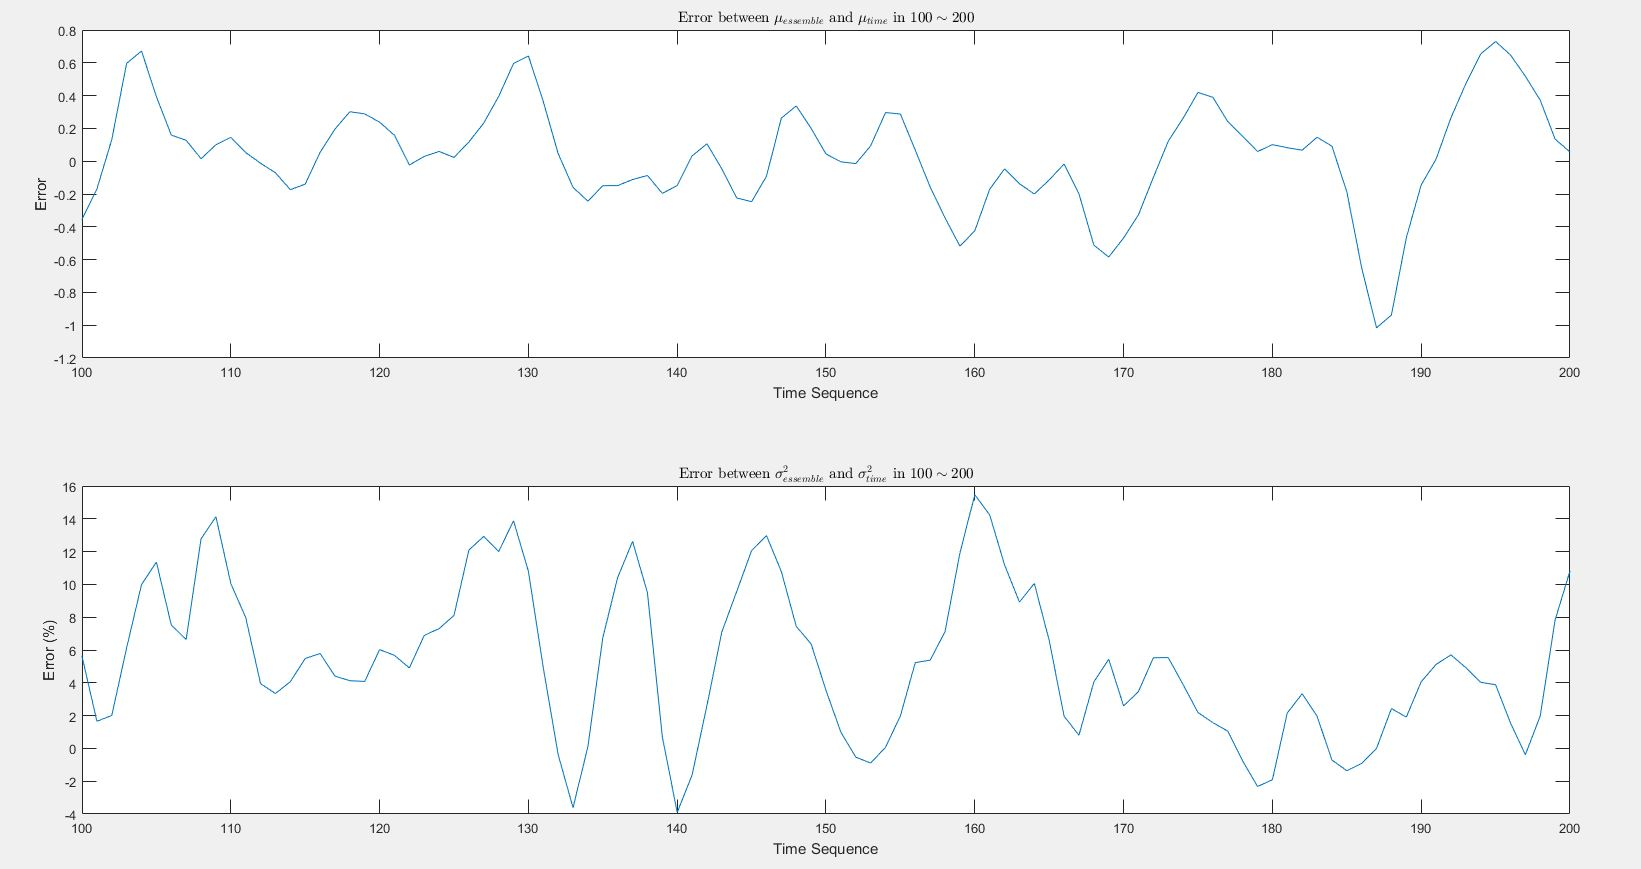
\includegraphics[scale=0.4]{Problem3d}
				\caption[Ensemble average and essemble variance with stationary part]{We can see the output signal is stationary by the both figures.The first one is based on the formula $\mu_{esemble}-\mu_{time}$ and the second one is based on $\frac{\sigma^{2}_{emsemble}-\sigma^{2}_{time}}{\sigma^{2}_{time}}$.}
			\end{figure}
			\begin{figure}[H]
				\centering
				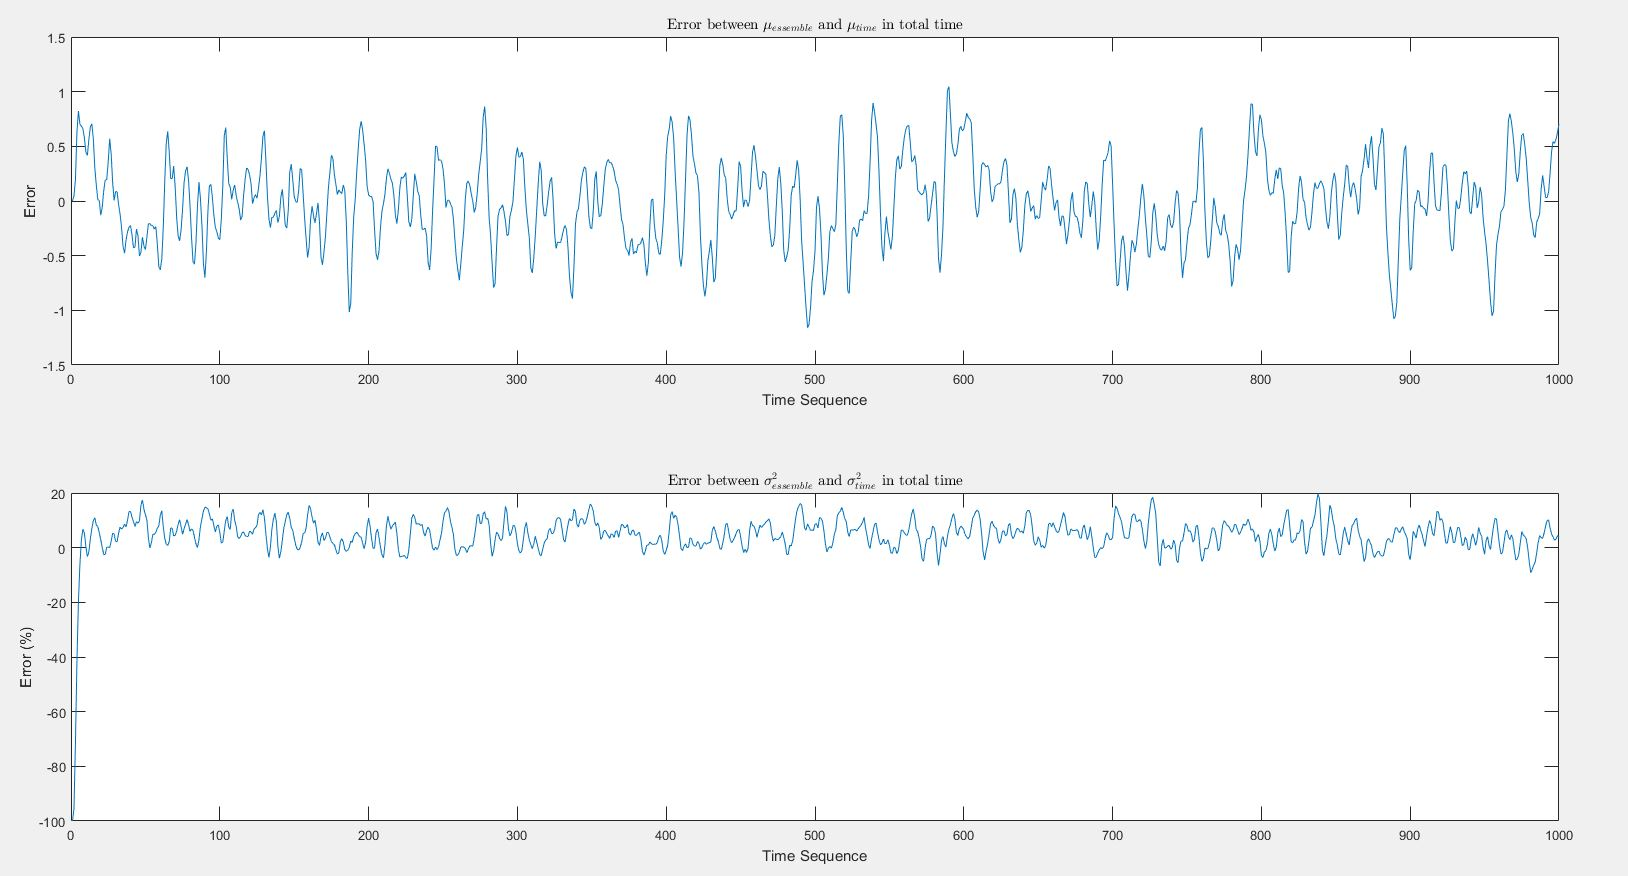
\includegraphics[scale=0.4]{Problem3e}
				\caption[Ensemble average and essemble variance for all time sequence]{Ensemble average and ensemble variance for all time sequence}
			\end{figure}
			\paragraph{If}we can't get the essembly statistical properties for stationary testing.We can use the follow steps to do stationary test:
				\begin{itemize}
					\item Divide the sample record into N equal sample time and the data in the sample time interval should be thought as independent.
					\item Compute the statistical properties likes mean,variance$\cdots$ separately and form a sequence.
					\item The elements in the sequences should be same as the total time statistical properties.
					\item Change the sample time and check again.
				\end{itemize} 
			\paragraph{If}we use the 20000 sequences to do stationary test and we define the sample time as 200.We can get a table like following one:\\
					\begin{table}[H]
						\scalebox{0.6}{
							
							\begin{tabular}[scale=0.5]{|c|c|c|c|c|c|c|c|c|c|c|}
								\hline
								Input singnal($\mu_{sample time}-\mu_{time}$)& 0.1791  &  0.8062  &  0.3819 &  -0.6777 &   0.6316 &   0.5150 &  -0.3552  & -0.8148 &   0.4015\\ \hline
								Ouput singnal from 1st filter($\mu_{sample time}-\mu_{time}$)& 0.1488   & 0.8176 &   0.3850 &  -0.6888 &   0.6977   & 0.5127 &  -0.3330  & -0.8581 &   0.4057
								\\ \hline
								Ouput singnal from 2nd filter($\mu_{sample time}-\mu_{time}$)& 0.1417  &  0.8188  &  0.3835 &  -0.7008 &   0.7046 &   0.5347 &  -0.3262  & -0.8675 &   0.3973\\ \hline
								Input Singnal ($\frac{\sigma_{sample time}^{2}-\sigma_{time}^{2}}{\sigma_{time}^{2}}$) \%&0.0421 &  -1.5080 &   5.6222 &   2.5148  & -3.5034  &  2.3513 &  -4.4475 &  -0.6911 &  -0.2100\\ \hline
								Ouput singnal from 1st filter ($\frac{\sigma_{sample time}^{2}-\sigma_{time}^{2}}{\sigma_{time}^{2}}$ ) \%&-1.0139  &  1.4121 &   1.8373 &   0.7246   & 0.4861 &  -0.8954  & -2.5458 &   0.0653 &  -1.1979\\ \hline
								Ouput singnal from 2nd filter ($\frac{\sigma_{sample time}^{2}-\sigma_{time}^{2}}{\sigma_{time}^{2}}$ )\%&-1.2052 &   1.8855 &   1.4090  &  0.4952 &   0.9871 &  -1.2865&   -2.5248 &   0.1202&   -1.5903\\
								\hline
							\end{tabular}
						}
						\caption[Statiscal properties of the input and output signal]{Statiscal properties of the input and output signal}
					\end{table}
			\paragraph{From}table 1 , we can think that either input or output are close to stationary.We can also use the other method like Wald–Wolfowitz runs test\cite{Book1}\cite{Net2}, we use the matlab run test function 'runtest' an the result are below:\\ 
				\begin{table}[H]
				\scalebox{0.6}{
					\centering
					\begin{tabular}[scale=0.5]{|c|c|c|}
						\hline
						Input&Ouput from 1st filter& Output from 2nd filter\\ \hline
						0&1&1\\ 
						\hline
					\end{tabular}
				}
				\caption[Result of run test for the input and output signal]{Result of run test for the input and output signal}
			\end{table}
			\paragraph{The} result $'0'$ means that the sequence is stationary at the 5\% significance level by the method.
	\section{Discussion}
		\subsection{Problem 1}
			\paragraph{Figure}one shows that the Gaussian white noise has the all properties which described by the equation $1\sim4.$Figure 2 shows the output of the Box-M\"{u}ller method from previous homework has the same result which means that the method is good for generating the Gaussian white noise.
		\subsection{Problem 2}
			\paragraph{Figure 6}shows that white properties are same as the result of the problem 1.Figure 7 and 8 show that the output of an LTI filter is still Gaussian distribution with the Gaussian white input.This property is the invariant property of the Gaussian white process.  However,we can notice that the white property will be destroyed by the filter from the autocorrelation and the autospectral density diagram . The trend of output signal's autospectral density function is accord with the equation 5 and equation 7.The corner frequency of these filter are close to the corner frequency of the Bode plot.This can be the proof of the the equation 5 and equation 7.
		\subsection{Problem 3}
		\paragraph{The} problem shows that the stationary ergodic can be checked by the equality of the time average and ensemble average.We can also check the ensemble variance(standard deviation) and the time variance(standard deviation) for testing stationary property. We can know that the output signal doesn't reach stationary form the essemble variance diagram of figure 15.We can use the stationary test method like run test,reverse arrangements test $\cdots$ to test the stationary of a sequence.
	\section{Appendix}
	\paragraph{All}of my code ca be found on the \href{URL}{Github.}
	\begin{itemize}
		\item Problem1a.m: Figure 1 \& 2
		\item Problem2a.m: Figure 4 \& 5
		\item Problem2b.m: Figure 6 $\sim$ 12
		\item Problem2c.m: Figure 13 $\sim$ 17
		\item Problem2d.m: Table 1 \& 2
	\end{itemize}
	\begin{thebibliography}{10}
		\bibitem{Book2}Roy D. Yates , David J. Goodman "Probability and
		Stochastic Processes
		A Friendly Introduction
		for Electrical and Computer Engineers"
		\bibitem{Book1}Julius S.Bendat , Allan G.Piersol "Random Data Analysis And Measurement Procedures"
		\bibitem{Net1} \href{https://en.wikipedia.org/wiki/Wiener%E2%80%93Khinchin_theorem}{Wiener-Khinchin theorem from Wikipedia}
		\bibitem{Net2} \href{https://en.wikipedia.org/wiki/Wald%E2%80%93Wolfowitz_runs_test}{Wald–Wolfowitz runs test from Wikipedia}
	\end{thebibliography}	
\end{CJK} 
\end{document} 
